%MARCOS RIAL DOCAMPO
%Parte del documento principal TFG

%%%%%%%%%%%%%%%%%%%%%%%%
%% MATERIAL Y MÉTODOS %%
%%%%%%%%%%%%%%%%%%%%%%%%


\chapter{Material y métodos}
\label{cap:materialymetodos}

%\minitoc
\section{Especies}
De todas las especies de mangle existentes en el Golfo de Fonseca se ha decidido tomar tres para este estudio por ser las más predominantes. Son las siguientes:

\begin{itemize}
	\item Mangle Rojo. Nombre científico \textit{Rhizophora mangle} \citep{JimenezRhizophora}.
	\item Mangle Blanco. Nombre científico \textit{Laguncularia racemosa} \citep{JimenezLaguncularia}.
	\item Mangle Prieto. Nombre científico \textit{Avicennia germinans} \citep{JimenezAvicennia}.
\end{itemize}

\section{Datos}
\label{sec:datos}
%\markboth{MATERIAL Y MÉTODOS}{DATOS}
Los datos obtenidos por el profesor Rafael Enrique Corrales con el espectro-radiómetro de campo se presentan en cuatro archivos de extensión .dat uno para cada especie más uno del conjunto que no se utilizará. Al abrir estos archivos en un editor de texto se puede observar como están compuestos por 
cuatro columnas de datos:

\begin{enumerate}
	\item Nombre. Columna opcional, en este caso será ``Subset 1''.
	\item Identificador compuesto por números enteros.
	\item Longitud de onda.
	\item Reflectividad.
\end{enumerate}

La característica principal de estos datos es que abarcan un amplio rango espectral de forma continuada, similar a lo que ocurre en la obtención de una imagen, pero en este caso los datos serían solamente de un punto, no de una superficie extensa.\Sep

%El rango espectral dado por el espectro-radiómetro comprende de 325 - 1075 nm que equivaldría a las cinco primeras bandas del \ac{OLI} de Landsat, es decir, aerosol, azúl, verde, rojo e \ac{IRC}. Teniendo en cuenta la realización de un corte de colas para que los datos sean lo más fiables posible.

\section{Software} \label{sec:software}
%\markboth{MATERIALES Y MÉTODOS}{SOFTWARE}
El uso de software libre es un recurso importante para realizar trabajos sobre recursos medioambientales principalmente por, entre otras cosas \citep{MatellanOliveira2004}:

\begin{enumerate}
	\item Abarata el coste del proyecto al ser bajo o nulo el coste de una licencia de uso.
	\item Cuenta con un buen soporte y servicio técnico llevado en algunos casos por comunidades de usuarios y a largo plazo. Se evita la obsolescencia del producto.
	\item Formatos estandarizados que permiten la interoperabilidad.
	\item Se centra en proporcionar un servicio y no un producto.
\end{enumerate}

Este \ac{TFG} se ha hecho íntegramente con software libre, utilizando los programas seguidamente mencionados sobre un sistema operativo GNU/Linux, en concreto sobre la distribución Ubuntu 14.04.\Sep

Adicionalmente se ha hecho un control de versiones remoto con el software Git (libre bajo licencia GNU GPL) que mediante repositorios, permite gestionar un historial de ficheros y carpetas, recordando y organizando el contenido en cada momento documentando los cambios que ha sufrido y quién y por qué los ha realizado. Permite, por tanto, recuperar el documento a versiones anteriores o revisar el proceso de desarrollo del mismo funcionando como respaldo. De esta forma se permite el acceso a los archivos por la plataforma web GitHub de forma pública. La interfaz gráfica utilizada ha sido SmartGit \citep{GmbH2015} libre y de uso gratuito para fines no comerciales y donde se pueden hacer cómodamente la mayoría de las operaciones de control de cambios.\Sep

Otra opción en lo que a control de versiones se refiere sería la del software \ac{SVN} \citep{Latex2011} pero este solamente permite hacer un control local de los cambios.

\subsection{R}
Para el tratamiento de los datos se ha utilizado el software estadístico de uso libre CRAN, más conocido como R \citep{R2013}. R se distribuye bajo licencia GNU GPL y puede definirse como un software de análisis estadísticos, como un generador de gráficos o como un lenguaje de programación. Si bien es un software pensado para su uso sobre interfaces de código, para la realización de este \ac{TFG} se ha utilizado la interfaz gráfica del software libre RStudio, bajo licencia AGPL, con el fin de hacer que su uso resulte más amigable.\Sep

R, como la mayoría de software que funciona sobre sistema operativo GNU/Linux, se compone de módulos o paquetes que se incorporan a una base del programa para extender sus posibilidades y funciones.\Sep

R es uno de los lenguajes más utilizados en estadística. Adicionalmente abarca otros muchos campos debido a la cantidad de librerías disponibles como tratamiento de imágenes satélite o clasificación supervisada.

\subsection{GRASS GIS}
Para el tratado de imágenes Landsat y su posterior clasificación se utiliza el programa de \ac{SIG} gratuito y de código abierto \ac{GRASS}, distribuido bajo licencia GPL \citep{GRASS_GIS_software}. Este es un potente software en lo que a utilización de manejo y análisis de información geoespacial se refiere. Su funcionalidad es similar a otros programas \ac{SIG} como QGIS, en los cuales, mediante extensiones aplicadas a la base del programa podemos ampliar sus funciones y adaptarlas a nuestras necesidades \citep{neteler2002open}. Como R, \ac{GRASS} se puede utilizar mediante una interface de código pero se optó por la aplicación de una interface gráfica de usuario que facilita y agiliza mucho el trabajo.\Sep

\subsection{\LaTeX}
En la redacción de este documento de memoria se empleó \LaTeX, el intérprete de \TeX, lenguaje y motor de composición de textos de bajo nivel potente y versátil especialmente indicado para elaborar documentos de texto de alta calidad tipográfica. \LaTeX, software libre bajo licencia LPPL, es un conjunto de macros escritas en lenguaje \TeX\ para la realización de múltiples tareas en lo que a la redacción de un documento de texto se refiere \citep{Latex2011} \citep{galindo2001} \citep{lamport1994}.\Sep

Como editor se utilizó TeXMaker \citep{Brachet2003} un entorno integrado de edición libre (licencia GPL) que facilita la redacción, edición, compilación y revisión del documento.\Sep

Para la gestión de la bibliografía, las referencias cruzadas y que fuera correctamente incluida en este documento se ha utilizado el software libre JabRef (licencia GPL). Este software compila la bibliografía mediante BibTeX, el formato estándar de bibliografía de \LaTeX.

\section{Técnicas de análisis espectral}
\label{sec:tecnicas}
%\markboth{MATERIALES Y MÉTODOS}{TÉCNICAS DE ANÁLISIS}

Las técnicas de separabilidad empleadas en este \ac{TFG} serán:
\begin{itemize}
	\item Codificación binaria e índice de acuerdo espectral.
	\item Clasificación angular.
	\item Continuum removal.
\end{itemize}

Se utilizarán para ello diversas funciones creadas en el lenguaje de programación R que se aplicarán a los datos tomados en campo.

\subsection{Índice de acuerdo espectral}
Con el fin de cuantificar de alguna forma la similitud entre los espectros de dos cubiertas a priori diferentes, podemos aplicar lo que se llama \ac{IAE} \citep{chuvieco2002teledeteccion}, que viene dado por la siguiente expresión:

\begin{equation} \label{eq:IAE}
	IAE = \frac{\sum_{k=1,m}(CB_{i,k} - CB_{j,k})^{2}}{m}
\end{equation}\Sep

Siendo $CB_{i,k}$ la codificación binaria del espectro \textit{i} para cada banda \textit{k}, $CB_{j,k}$ la codificación binaria del espectro \textit{j} para cada banda \textit{k} y \textit{m} el número de bandas.\Sep

Este método de cuantificación está basado en una codificación binaria (0 y 1) del espectro para cada banda. Cuanto más cercano sea el valor del \ac{IAE} a 0, los espectros serán más similares, al contrario que cuanto más se aproxime el valor a 1. De esta forma no solo se puede obtener un análisis cuantitativo de la similitud entre dos espectros, sino que también podremos realizar un análisis a simple vista realizando gráficas de la clasificación binaria de cada espectro.\Sep

En la figura \ref{fig:IAE} se muestra el script de la función en R a la que se le aplicarán los datos de campo y que devuelve el dato de acuerdo espectral.

\begin{figure}
\centering
\begin{lstlisting}[language = R, frame = single]
  IAE <- function(i, j) {
  
  mediai = mean(i$V5)
  CBi = sapply(i$V5, FUN=function(x) {if(x>=mediai) {1} else {0}})
  
  mediaj = mean(j$V5)
  CBj = sapply(j$V5, FUN=function(x) {if(x>=mediaj) {1} else {0}})
  	
  Indice = sum((CBi-CBj)^2)/length(CBi)
  return(Indice)  
}
\end{lstlisting}
\captionsetup{font={footnotesize,it}}
\caption[Función de Índice de Acuerdo Espectral]{Script de la función del Índice de Acuerdo Espectral en R. Fuente: Elaboración propia.}
\label{fig:IAE}
\end{figure}

\subsection{Continuum removal}
\label{subsec:Continuum_removal}

El método de \ac{CR} o, como lo cita \cite{chuvieco2002teledeteccion}, análisis de absorción diferencial frente a la tendencia, es una técnica de análisis en la que se marcan en cada observación los valores máximos relativos o locales de reflectividad. Estos máximos sirven como indicadores de tendencia de la observación. Esta técnica busca eliminar el efecto de albedo, permitiendo centrar el análisis en la absorción diferencial propia de cada banda. Lo analizado principalmente será la intensidad de la absorción o profundidad en cada sección de la gráfica, así como la asimetría y anchura con el fin de detectar similitudes entre dos o más muestras espectrales. Fue utilizado por primera vez en 1999 por Kokaly y Clark.\Sep

\cite{huang2004estimating} testaron la efectividad de esta técnica para estimar el contenido de substancias químicas en hojas (de donde se extraen los ejemplos de la figura \ref{fig:ejemploCR}). En otro ejemplo \cite{filippi2007effect} emplean el \ac{CR} como utilidad para realizar clasificaciones de vegetación con imágenes hiperespectrales. Y \cite{underwood2003mapping} utiliza este método para detectar y determinar el impacto de especies forestales invasoras sobre otras especies autóctonas apoyándose también en imágenes hiperespectrales.

\begin{figure}
	\centering
	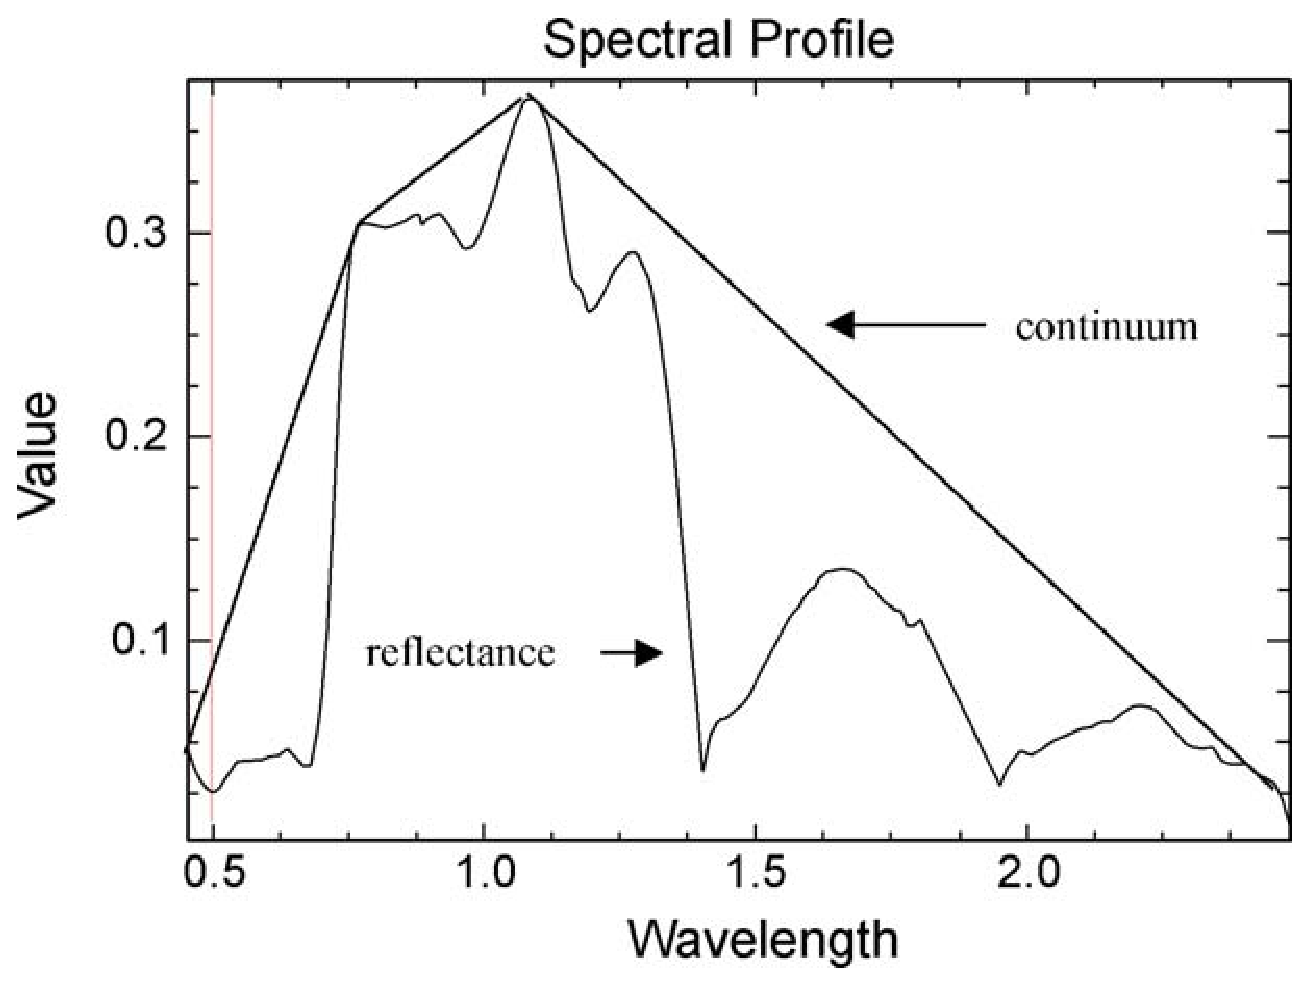
\includegraphics[width=0.5\linewidth]{./Imagenes/CR1.eps}
	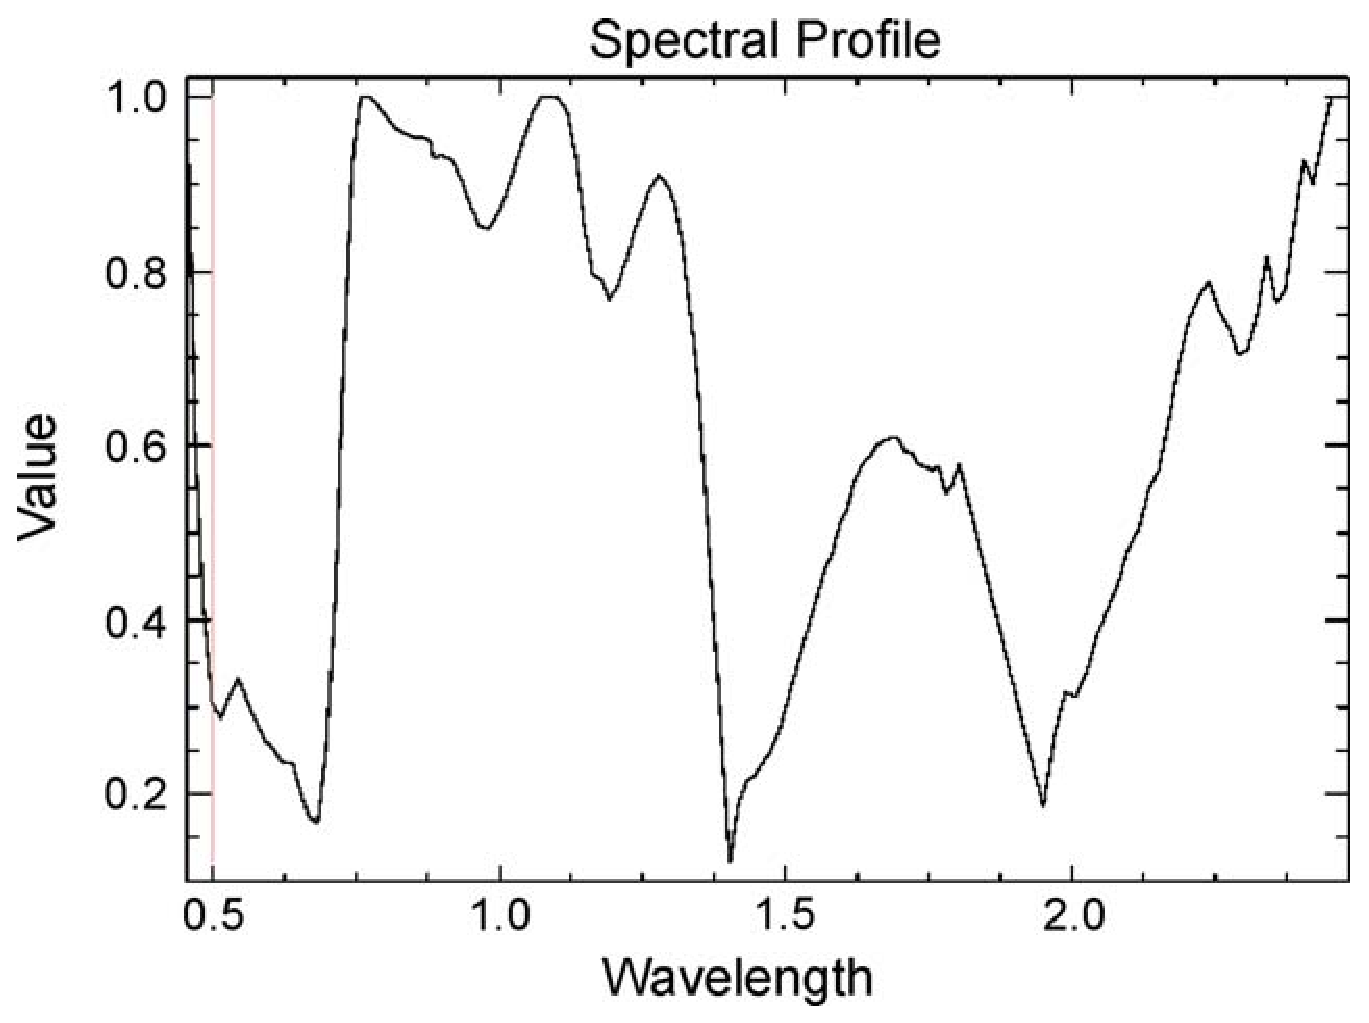
\includegraphics[width=0.5\linewidth]{./Imagenes/CR2.eps}
	\captionsetup{font={footnotesize,it}}
	\caption[Continuum Removal ejemplo]{Ejemplo de aplicación de la técnica continuum removal. Fuente: Extraído de \cite{huang2004estimating}.}
	\label{fig:ejemploCR}
\end{figure}

Este método no aporta un valor numérico de cuantificación de la similitud entre dos espectros, centrándose en un análisis gráfico de cada respuesta por separado.\Sep

El paquete base de R ya incluye las operaciones estadísticas básicas necesarias para la elaboración de la clasificación angular y el \ac{IAE} con la única excepción de que para poder aplicar el analizador \ac{CR} se debe descargar el paquete adicional \textit{prospectr} \citep{stevens2014introduction}.\Sep

En la figura \ref{fig:CR} se muestra el script de la función en R a la que se le aplicarán los datos de campo y que devuelve la gráfica de \ac{CR}.

\begin{figure}
\centering
\begin{lstlisting}[language = R, frame = single]
require(prospectr)

cr <- continuumRemoval(mangle1corte$V5, mangle1corte$V4, type="R",
			interpol="linear")
grafica(data1)
lines(data1$V4,cr)
\end{lstlisting}
\captionsetup{font={footnotesize,it}}
\caption[Función de Continuum Removal]{Script de la función de Continuum Removal en R. Fuente: Elaboración propia a propia a partir de \cite{stevens2014introduction}.}
\label{fig:CR}
\end{figure}

Se puede observar como mediante el comando \textit{``require()''} se llama al paquete \textit{prospectr}, que debe estar instalado para que el script funcione correctamente. Para ello se utilizó el instalador de paquetes de RStudio, localizando el paquete requerido en el repositorio oficial de RCRAN e instalando las dependencias necesarias, que también se podría haber hecho con el comando \textit{``install.packages()''}. El comando \textit{``grafica()''} es la llamada a una función creada para presentar la gráfica a nuestro gusto, mientras que con el comando \textit{``lines()''} se nos permite superponer la gráfica de \ac{CR} a la anterior.

\subsection{Clasificación angular}
La clasificación angular calcula la similitud entre dos espectros a partir de su distancia angular espectral. Originalmente este método compara espectros desconocidos con otros de referencia tomados, por ejemplo, de bibliotecas espectrales o de la misma imagen \citep{girouard2004validated} con el fin de asignar píxeles desconocidos a clases de referencia conocida en una clasificación temática. El algoritmo de clasificación angular es el siguiente:

\begin{equation} \label{eq:angular}
	\theta = arcos \frac{\sum_{k=1}^{m} \rho_{i,k} \rho_{j,k}}{\sqrt{\sum_{k=1}^{m} \rho_{i,k}^{2}} \sqrt{\sum_{k=1}^{m} \rho_{j,k}^{2}}}
\end{equation}\Sep

Siendo $\rho_{i,k}$ la reflectividad del espectro \textit{i} en una banda \textit{k}, $\rho_{j,k}$ la reflectividad del espectro \textit{j} en la misma banda y \textit{m} el número de bandas.\Sep

Los espectros serán más similares cuanto menor sea el valor del ángulo $\theta$ de la ecuación \ref{eq:angular}.\Sep

En la figura \ref{fig:AE} se muestra el script de la función en R a la que se le aplicarán los datos de campo y que devuelve el valor del ángulo $\theta$.

\begin{figure}
\centering
\begin{lstlisting}[language = R, frame = single]
AE <- function(i,j) {
  
  Ri = i$V5
  Rj = j$V5

  Angulo = acos (sum(Ri*Rj)/(sqrt(sum(Ri^2))*sqrt(sum(Rj^2))))
  return(Angulo)
}
\end{lstlisting}
\captionsetup{font={footnotesize,it}}
\caption[Función clasificación angular]{Función de clasificación angular en R. Fuente: Elaboración propia.}
\label{fig:AE}
\end{figure}

\section{Imágenes de satélite}
\subsection{Landsat 8}
Landsat 8 dispone de 11 bandas espectrales: 9 del sensor \ac{OLI} (expuestas en la tabla \ref{tab:sensoresOLI}) y 2 del sensor \ac{TIRS} que no son de interés para este trabajo.\Sep

Como los datos del radiómetro de campo solo abarcan las longitudes de onda comprendidas entre $325 nm$ y $1075 nm$ solo son de interés las cinco primeras bandas que se detallan a continuación:

\begin{itemize}
	\item Banda 1 (Coastal/Aerosol) [430-450 nm]: Detecta azules y violetas intensos. Solventa los problemas de la dispersión de Rayleigh. Facilita la detección de la calidad de aguas poco profundas y partículas de polvo o aerosol en la atmósfera.
	\item Banda 2 (Blue) [450-510 nm]: Detecta el azul del espectro visible. Útil para diferenciar el suelo desnudo de la vegetación y detectar zonas pavimentadas como carreteras o áreas urbanas.
	\item Banda 3 (Green) [530-590 nm]: Detecta el verde del espectro visible. Sensible al nivel de turbidez del agua. Brillante en zonas de tierra árida y oscura en zonas boscosas o de cultivos.
	\item Banda 4 (Red) [640-670 nm]: Detecta el rojo del espectro visible. Útil en la clasificación de zonas vegetales pero no diferencia estas de agua, puesto que aparecen como zonas oscuras.
	\item Banda 5 (NIR) [850-880 nm]: Detecta el infrarrojo cercano. Especialmente importante en ecología porque la vegetación vigorosa la refleja. Útil para la obtención del \ac{NDVI} y distinguir tipos de vegetación.
\end{itemize}


\subsection{Obtención de las imágenes}
Las imágenes se obtuvieron del servicio Earth Explorer, de la \ac{EROS} de la \ac{USGS}. Estas imágenes ya vienen con una corrección geométrica previa hecha, por lo que no será necesario aplicar más correcciones de este tipo. En un archivo .txt asociado a las imágenes .tiff para cada banda se especifica que el método de corrección geométrica utilizado ha sido el de convolución cúbica.\Sep

En concreto, los archivos que nos ofrece el servicio de descargas son:

\begin{itemize}
	\item Una imagen en composición de color natural como las que se muestran en la figura \ref{fig:imagenesLandsat}.
	\item Una imagen térmica que no nos será de utilidad.
	\item Una imagen de 8 bits que cuantifica la calidad de la observación.
	\item Las imágenes anteriormente citadas georreferenciadas.
	\item Las imágenes correspondientes a cada banda de Landsat 8 con la corrección geométrica aplicada (level 1) en formato GeoTIFF.
\end{itemize}\Sep

Se trata de un producto de \ac{L1T} con correcciones geométricas sistemáticas aplicadas utilizando para ello puntos de control terrestre o información de posición integrada a bordo \citep{Ariza2013}. Se entrega así una imagen registrada a la proyección WGS84. Adicionalmente en este nivel de producto contiene una corrección topográfica por el desplazamiento del terreno debido al relieve. Las imágenes se encuentran en formato de \ac{ND} que se pueden transformar a valores de reflectividad \ac{TOA} en las bandas 1 a 9.\Sep

Otra forma de obtener las imágenes de Landsat 8 es mediante el gestor de descargas Libra, que aprovecha la API del servicio de \ac{AWS} que aloja estas imágenes desde septiembre de 2014. Este nos permite elegir que bandas descargar, ahorrando tiempo en la operación.\Sep

En cambio, para la correcta realización de este \ac{TFG} donde tenemos datos de reflectividad a nivel del suelo, necesitamos que las imágenes Landsat también muestren valores de reflectividad a ese nivel. Esto se consigue aplicando un algoritmo de corrección radiométrica a las imágenes \ac{L1T} obteniendo un producto también proporcionado por la agencia \ac{EROS} bajo demanda llamado \ac{PL8SR} \citep{USGS2015}.\Sep

Para abarcar la zona de estudio se necesitaron obtener dos imágenes que tienen las siguientes características:

\begin{table}[ht]
	\centering
	\caption[Caracerísticas de las imágenes Landsat]{Características de las imágenes Landsat obtenidas (figura \ref{fig:imagenesLandsat}).}
	\begin{tabular}{|c|c|c|c|c|c|c|c|}
	\hline
	IMAGEN & PATH & ROW & FECHA & WEST & EAST & NORTH & SOUTH \\
	\hline
	1 (a) & 18 & 51 & 23/11/2014 & -89.105062 & -86.987819 & 14.067713 & 11.946409 \\
	\hline
	2 (b) & 17 & 51 & 19/12/2014 & -87.549399 & -85.443030 & 14.062287 & 11.952632 \\
	\hline
	\end{tabular}
	\label{tab:imagenes}
\end{table}

%Se observa en la tabla \ref{tab:imagenes} que la cobertura nubosa de la segunda imagen es elevada, pero en la zona de estudio, que ocupa un pequeño porcentaje de esta imagen, la cobertura es aceptable. Este hecho también se observa en las imágenes de calidad (figura \ref{fig:imagenescalidad}) en las que las nubes y nubes altas se marcan de color blanco y amarillo respectivamente.\Sep

Se consideró que el desfase temporal entre ambas imágenes y la fecha de toma de datos no era determinante suponiendo un escaso cambio fenológico de las especies de mangle en ese periodo de tiempo.\Sep

\begin{figure}
	\centering
	\subfloat[Imagen Landsat path 18 row 51 (23/11/14)]{
	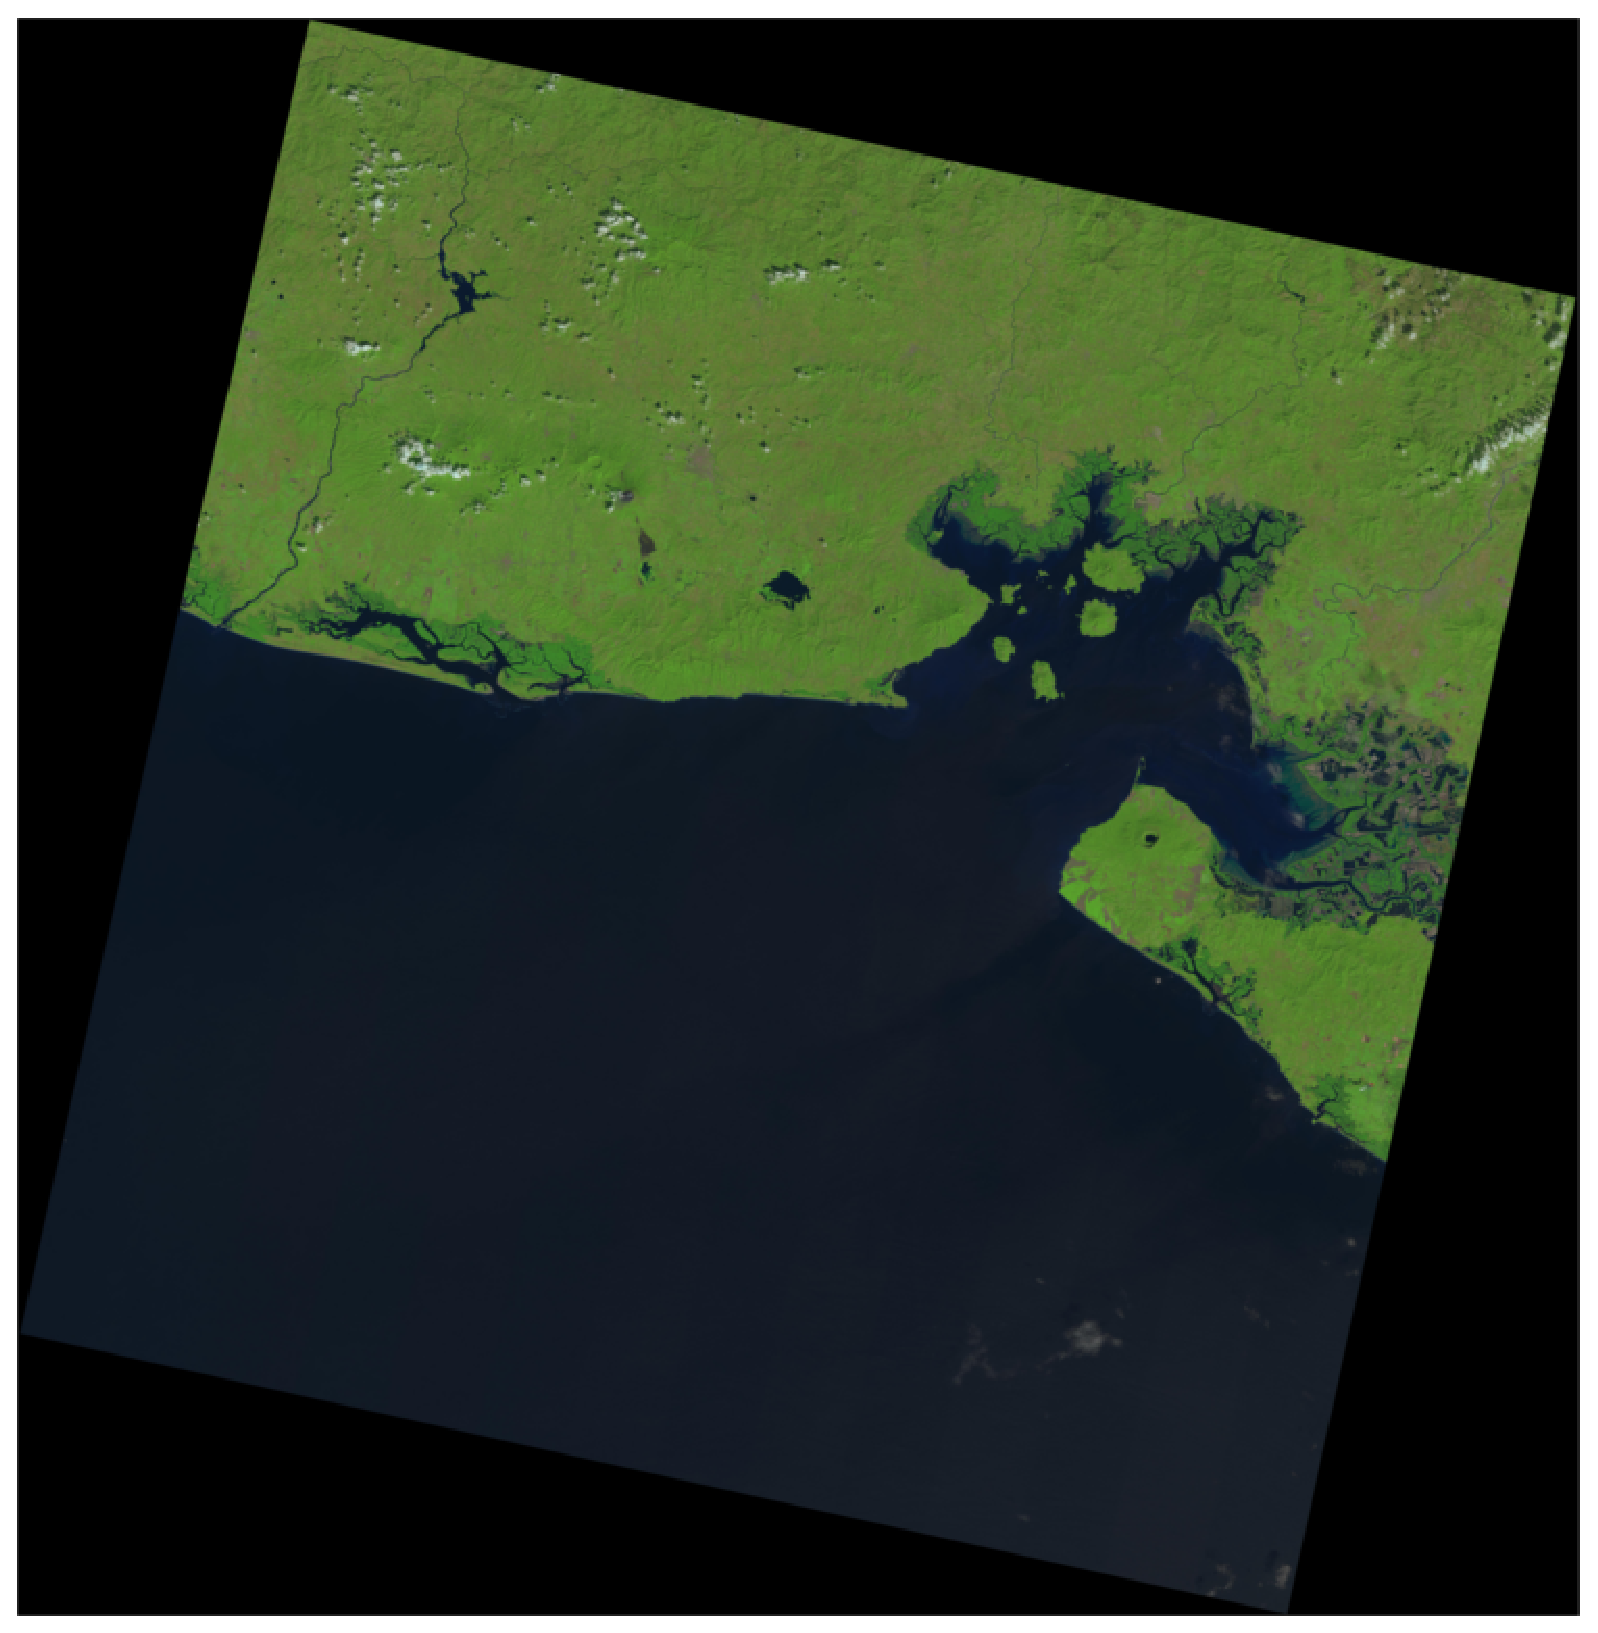
\includegraphics[width=0.4\linewidth]{./Imagenes/Landsat18.eps}}
	\subfloat[Imagen Landsat path 17 row 51 (19/12/14)]{
	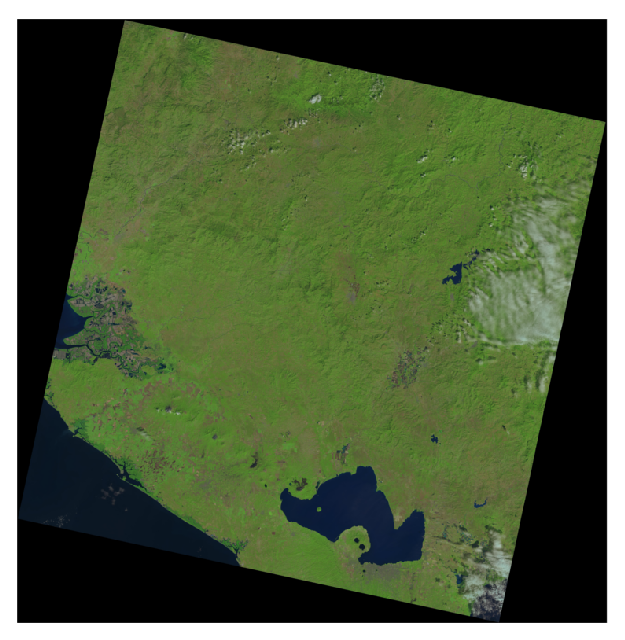
\includegraphics[width=0.4\linewidth]{./Imagenes/Landsat17.eps}}
	\captionsetup{font={footnotesize,it}}
	\caption[Imágenes Landsat]{Imágenes Landsat con corrección geométrica utilizadas para el trabajo. Fuente: USGS.}
	\label{fig:imagenesLandsat}
\end{figure}

\begin{figure}
	\centering
	\subfloat[Imagen de calidad Landsat path 18 row 51 (06/10/14)]{
	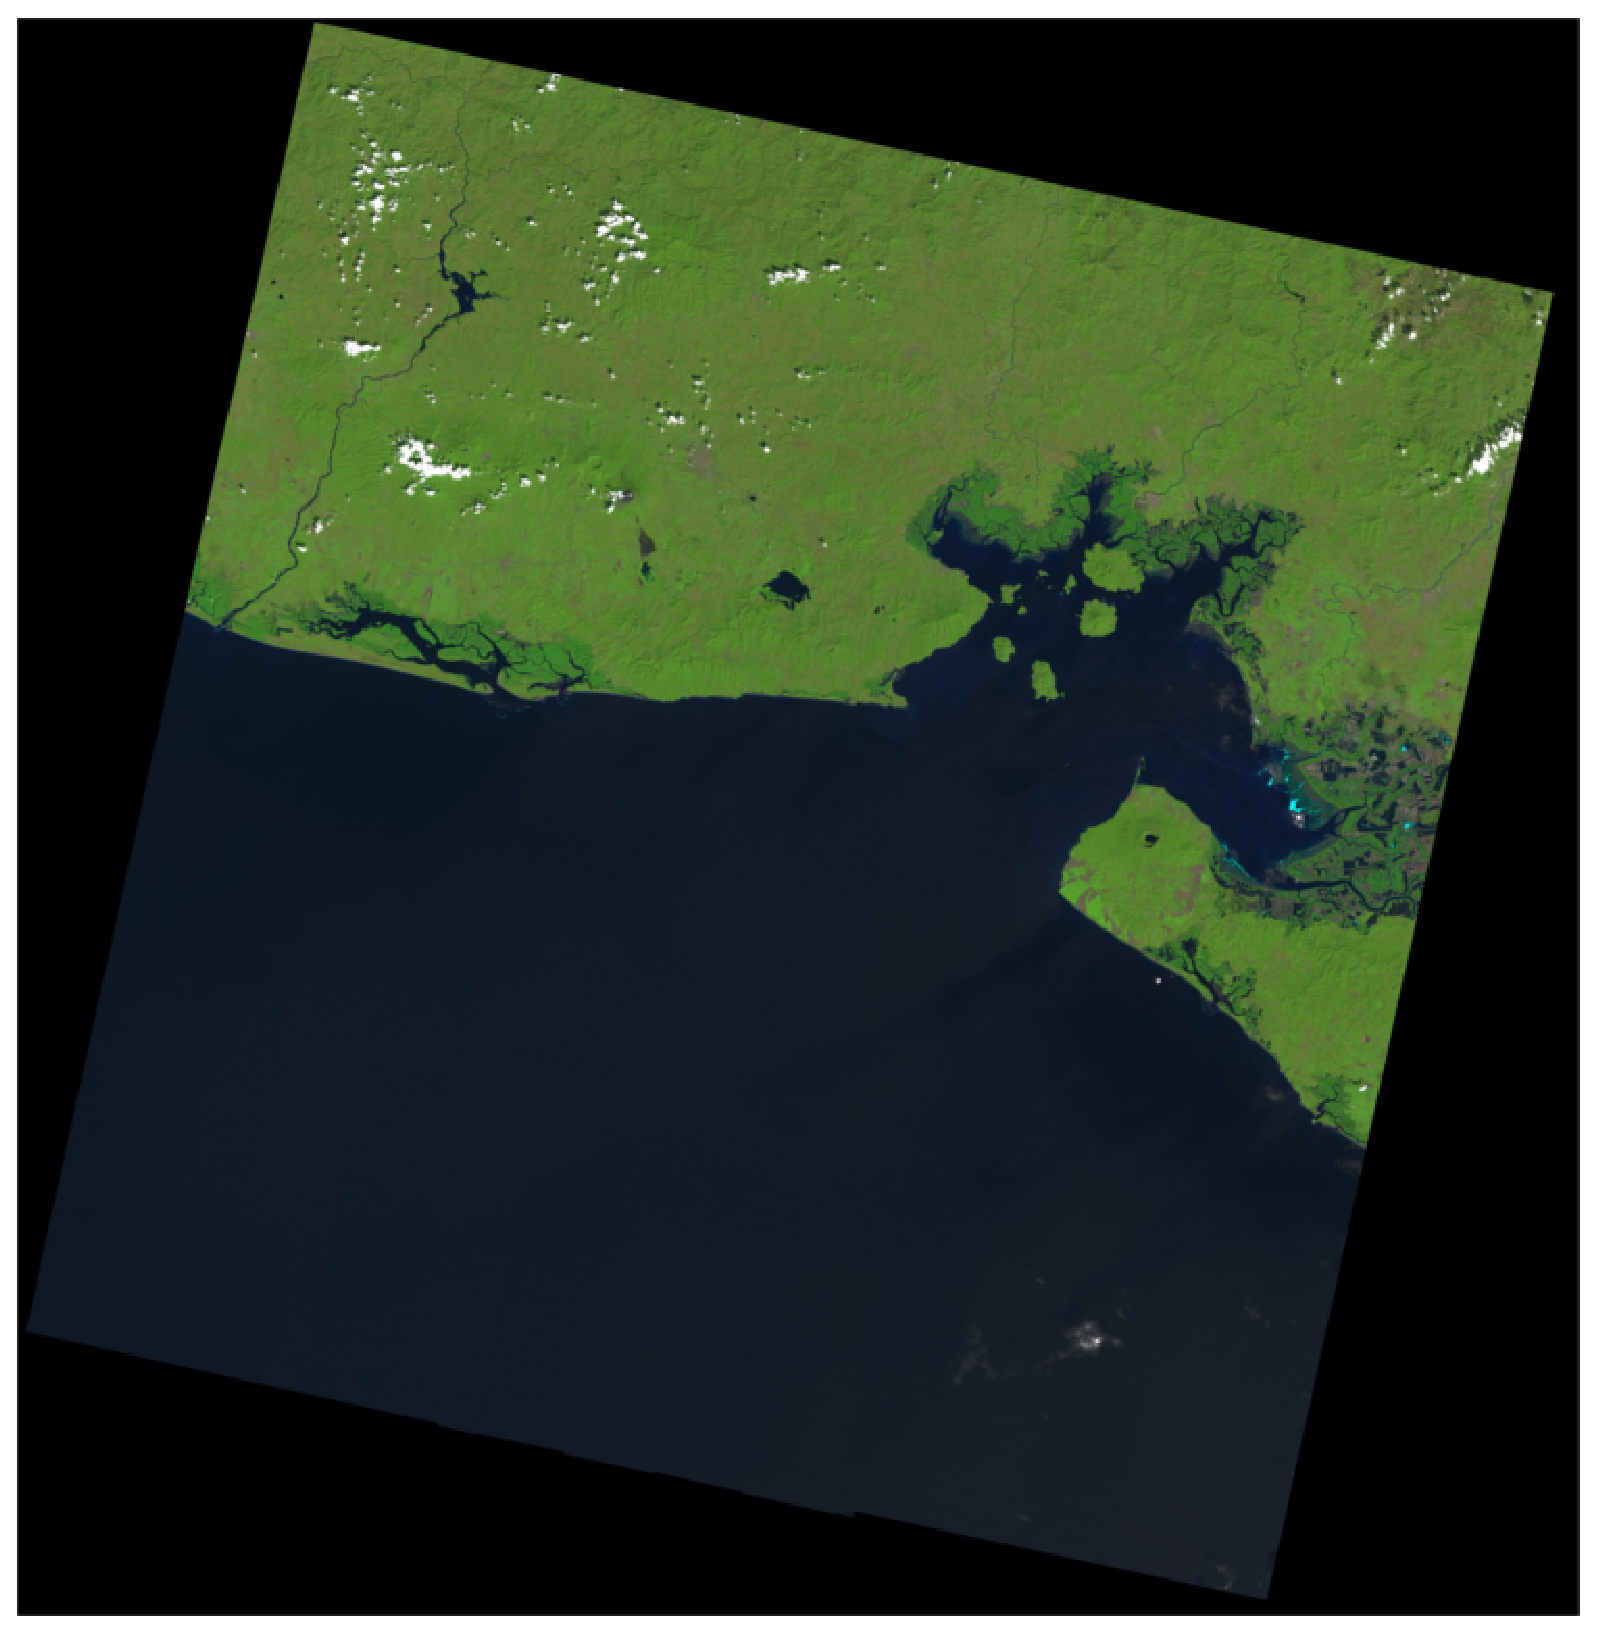
\includegraphics[width=0.4\linewidth]{./Imagenes/LandsatQ18.eps}}
	\subfloat[Imagen de calidad Landsat path 17 row 51 (16/11/14)]{
	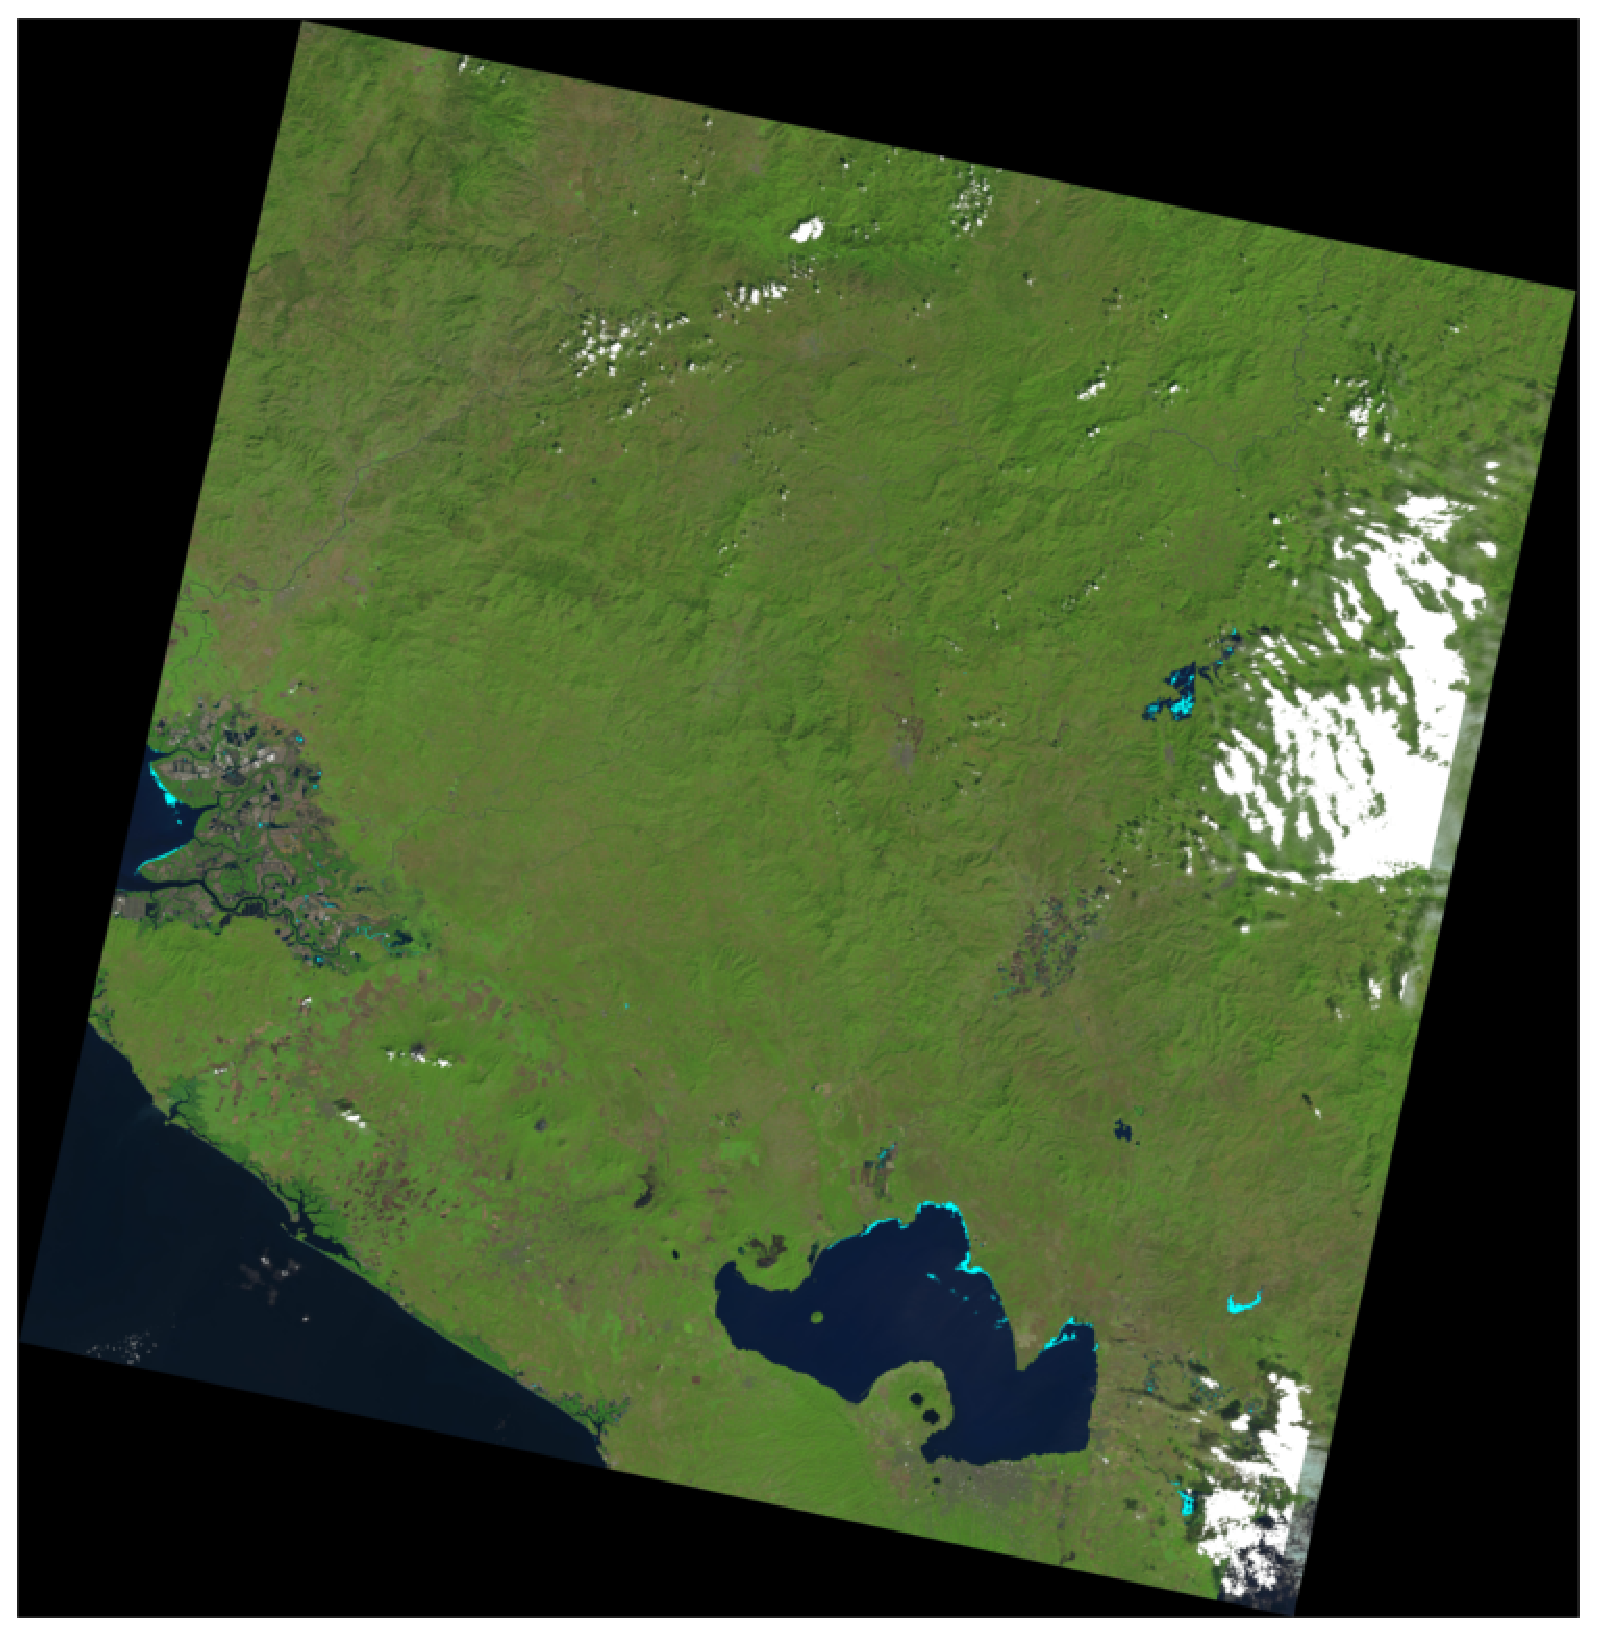
\includegraphics[width=0.4\linewidth]{./Imagenes/LandsatQ17.eps}}
	\captionsetup{font={footnotesize,it}}
	\caption[Imágenes de calidad de Landsat]{Imágenes de calidad de Landsat de 8 bits. Fuente: USGS.}
	\label{fig:imagenescalidad}
\end{figure}

Las imágenes utilizan el siguiente código de identificación en el nombre \citep{Ariza2013} \citep{USGS2015}

\begin{center}
	\fbox{LXSPPPRRRYYYYDDDGSIVV}
\end{center}

donde:

\begin{itemize}
	\item L: Landsat.
	\item X: Sensor.
	\item S: Satélite.
	\item PPP: Path.
	\item RRR: Row.
	\item YYYY: Año de adquisición de la imagen.
	\item DDD: Día juliano del año.
	\item GSI: Identificador de la estación terrestre de seguimiento.
	\item VV: Versión del archivo.
\end{itemize}

\subsection{Tratamientos previos}
Como se decía en el apartado anterior, la geometría de las imágenes ya está corregida. Pero es necesario realizar algunos procedimientos antes de unirlas y recortarlas finalmente para que se adapten a la zona de estudio y sea más cómodo trabajar con ellas. Estos procedimientos son el tratamiento de los valores nulos y la transformación de los \ac{ND} en reflectancias.\Sep

Lo primero que se debe hacer en GRASS es crear la localización de nuestro proyecto y añadir las imágenes al directorio de mapas. Los datos de la localización se establecen gracias a la lectura por parte de GRASS de la configuración de proyección y datum de un archivo de datos georreferenciado, es decir, de cualquier imagen de Landsat del trabajo.

\subsubsection{Valores nulos}
El tratamiento de los valores nulos se lleva a cabo mediante el comando ``r.null'' como sigue:

\begin{center}
\begin{boxedverbatim}
	r.null map=LC80180512014279LGN00_B1@TFG setnull=0 null=-9999
\end{boxedverbatim}
\end{center}

donde \textit{``map''} corresponde a la banda a tratar seguido por el \textit{mapset}, \textit{``setnull''} indica el valor de los elementos nulos y \textit{``null''} indica el nuevo valor de estos elementos. Se elige un valor de -9999 para evitar posibles errores de realizarse, por ejemplo un \ac{NDVI} que trabaja con valores de píxel de [-1,1].

\subsubsection{Transformación a reflectancias}
Los \ac{ND} pueden ser reescalados a valores de reflectancias \ac{TOA} gracias a los coeficientes radiométricos provistos en el archivo .txt que acompaña a las imágenes. Esta transformación se hará con el comando i.landsat.toar como sigue:
\begin{center}
\begin{boxedverbatim}
	i.landsat.toar
	input_prefix=LC80170512014320LGN00_B
	output_prefix=LC80170512014320LGN00_TOAR_B
	metfile=/home/marcos/grassdata/Imagenes/Landsat/
	P17R51/Base/LC80170512014320LGN00_MTL.txt
	sensor=oli8
	method=dos4
	date=2014-11-16
	sun_elevation=52.01756824
\end{boxedverbatim}
\end{center}

donde \textit{``input\_prefix''} es el prefijo del nombre de las imágenes para cada banda, \textit{``output\_prefix''} es el prefijo que le queremos dar a las nuevas imágenes corregidas, \textit{``metfile''} es el archivo de metadatos asociado, \textit{``sensor''} el tipo de sensor, \textit{``date''} es la fechas de adquisición y \textit{``sun\_elevation''} la elevación en grados del Sol.

\subsubsection{Mosaico de imágenes}
Para realizar el mosaico de las dos imágenes de las que disponemos tenemos dos opciones: utilizando la herramienta \textit{gdal\_merge.py} y hacerlo en GRASS. Para utilizar la herramienta de la librería \ac{GDAL} gdal\_merge.py debemos tener las siguientes consideraciones:

\begin{itemize}
	\item Es un método que se ejecuta en la terminal de Linux. Para un método guiado se utilizaría, por ejemplo, la herramienta \textit{raster/combinar} en QGIS o el método de GRASS que se expondrá más adelante.
	\item Las dos imágenes deben estar en el mismo sistema de coordenadas.
	\item Utiliza como método de remuestreo el de vecino más próximo.
	\item La última imagen de la lista será copiada sobre la precedente en el caso de haber solape.
\end{itemize}

La línea de comando en cuestión es la siguiente (para las imágenes de la primera banda y en el caso de tener situadas las imágenes en la misma carpeta):

\begin{center}
\begin{boxedverbatim}
	gdal_merge.py -n 0 -v LC80170512014320LGN00_B1.TIF 
	LC80180512014279LGN00_B1.TIF -o mosaico1.tif
\end{boxedverbatim}
\end{center}

En este caso se utilizan los comandos asociados u opciones siguientes: -n para que se ignoren los píxeles con valores nulos, -v para que se detallen las operaciones realizadas y -o que permite dar nombre al archivo de salida. Con este método no sería necesario realizar el tratamiento de valores nulos.\Sep

En la figura \ref{fig:dialogomosaico} se observa el diálogo resultante de la operación anterior que confirma que se ha hecho bien el mosaico. En el tenemos datos de las imágenes como el nombre, las coordenadas de la esquina superior izquierda e inferior derecha, tamaño del píxel y tiempo que se necesitó para realizar la operación.\Sep

\begin{figure}
	\centering
	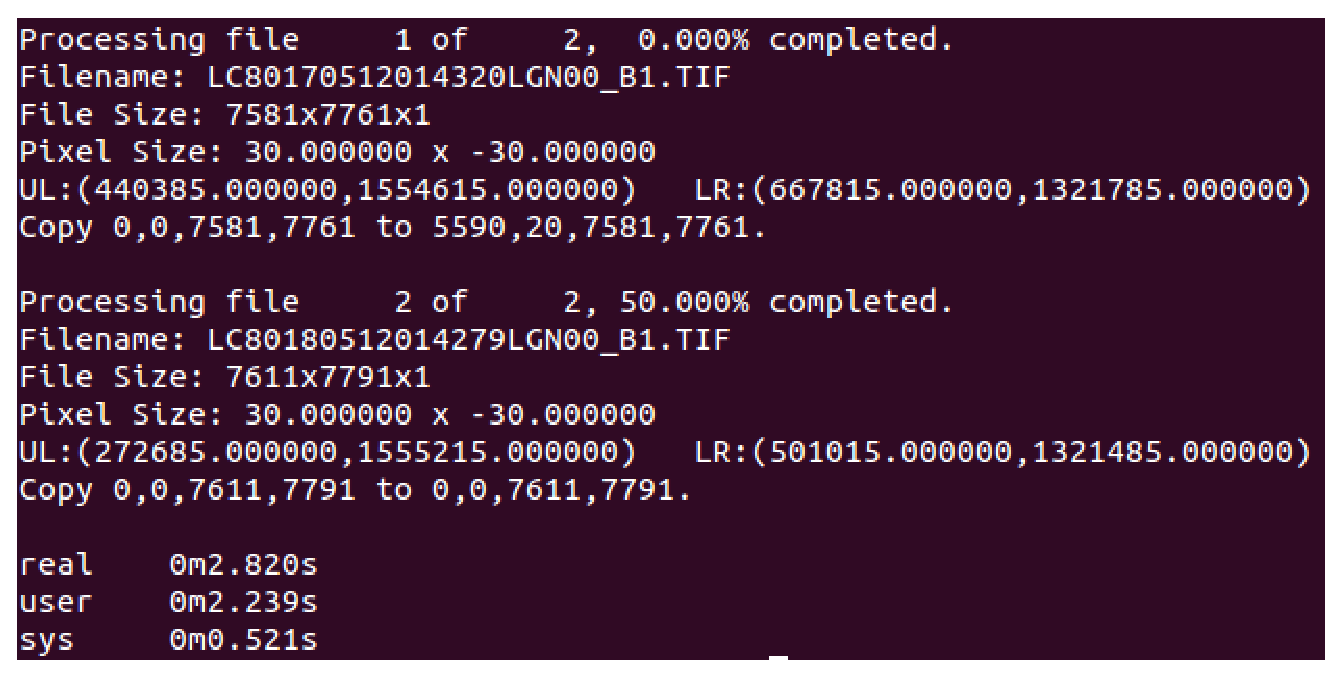
\includegraphics[width=0.8\linewidth]{./Imagenes/Dialogo_mosaico.eps}
	\captionsetup{font={footnotesize,it}}
	\caption[Diálogo del mosaicado]{Diálogo resultante del mosaicado de las imágenes. Fuente: Elaboración propia.}
	\label{fig:dialogomosaico}
\end{figure}

De hacerlo en GRASS, el comando sería \textit{r.patch}, con la salvedad de que las dos imágenes deben estar en la misma región de cálculo, la cual se puede ver en el cuadro \ref{tab:region}), quedando la siguiente línea de orden:\SmallSep

\begin{center}
\begin{boxedverbatim}
	r.patch image1=LC80180512014279LGN00_TOAR_B1@PERMANENT
	image2=LC80170512014320LGN00_TOAR_B1@PERMANENT
\end{boxedverbatim}
\end{center}

\subsubsection{Recorte de la imagen}
Para trabajar solamente con la zona de estudio es necesario recortar la imagen o reducir la región de cálculo. Para ello empleamos las opciones de visualización de GRASS con una extensión de coordenadas superior derecha de (516000 , 1501230) e inferior izquierda de (377940 , 1412100) como se muestra en el cuadro \ref{tab:region}. Una vez fijada se selecciona la opción de zoom ``set computational region from display extent'' que simplemente reduce la región de cálculo previamente establecida a la extensión de la visualización actual y nos permite realizar operaciones en esta.\Sep

\begin{table}[ht]
	\centering
	\caption[Datos de las regiónes de trabajo]{Datos de las regiónes de trabajo establecidas en GRASS.}
	\begin{tabular}{|r|c|c|}
	\hline
	& Extensión imágenes & Extensión reducida\\
	\hline
	Proyección & 1 (UTM) & 1 (UTM) \\
	\hline
	Zona & 16 & 16 \\
	\hline
	Datum & WGS84 & WGS84 \\
	\hline
	Elipsoide & WGS84 & WGS84 \\
	\hline
	Norte & 1555215 &1501230 \\
	\hline
	Sur & 1321485 & 1412100 \\
	\hline
	Oeste & 272685 & 377940 \\
	\hline
	Este & 667815 & 516000 \\
	\hline
	Res. esp. vertical (m) & 30 & 30 \\
	\hline
	Res. esp. horizontal (m) & 30 & 30\\
	\hline
	Filas & 7791 & 2971 \\
	\hline
	Columnas & 13171 & 4602 \\
	\hline
	Celdas & 102615261 & 13672542 \\
	\hline
	\end{tabular}
	\label{tab:region}
\end{table}

Con el comando \textit{r.resample} se hace el remuestreo mediante vecino más próximo del área del recorte permitiendo obtener la imagen final para cada banda (figura \ref{fig:recorte}). El comando se emplea de la siguiente forma para cada banda:

\begin{center}
\begin{boxedverbatim}
	r.resample input=MosaicoB1@TFG output=L8GF_SRB1
\end{boxedverbatim}
\end{center}

\begin{figure}
	\centering
	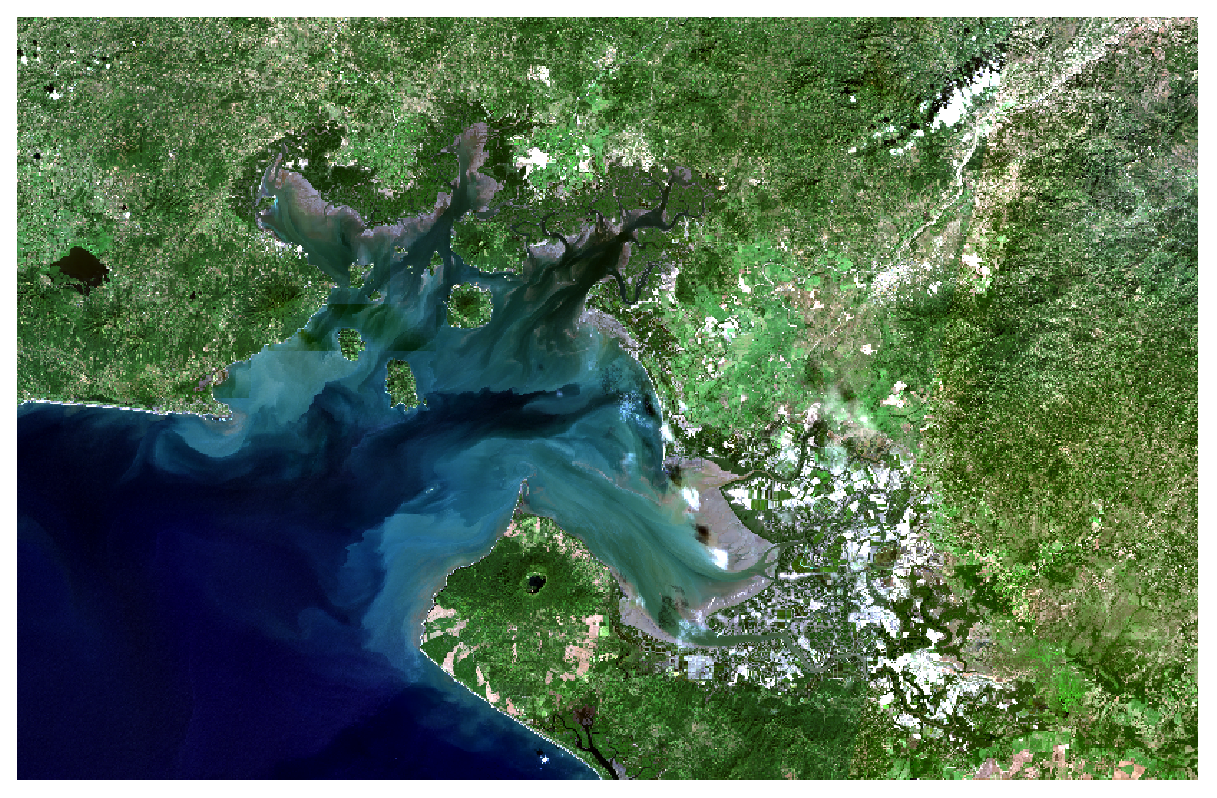
\includegraphics[width=0.8\linewidth]{./Imagenes/Recorte.eps}
	\captionsetup{font={footnotesize,it}}
	\caption[Recorte de imagen Landsat]{Resultado del recorte de la imagen. Imagen exportada de GRASS. Fuente: Elaboración propia.}
	\label{fig:recorte}
\end{figure}

\subsubsection{Filtro de media}

\section{Estudio radiométrico}